\documentclass[twoside,11pt,a4paper,openright]{article}
\usepackage[utf8]{inputenc}
\usepackage{amsmath}
\usepackage{listings}
\usepackage{pdfpages}
\usepackage{amsfonts}
\usepackage{caption}
%\usepackage{cite}
\usepackage{amssymb}
\usepackage[english]{babel}
\usepackage{fancyhdr}
\usepackage{graphicx}
%\usepackage{comment}
\usepackage{siunitx}
\usepackage{changepage}
\usepackage[rmargin=3cm,tmargin=3cm]{geometry}
%\usepackage[toc,page]{appendix}
%\usepackage{natbib}
%\usepackage{dsfont}
\usepackage{mathrsfs}
\usepackage{epstopdf}
\usepackage[labelfont=bf,width=0.92\textwidth]{caption}
% \usepackage{mathtools}
% \usepackage{breqn}
\usepackage{pbox}
\usepackage{upgreek}
\usepackage{epstopdf}
\usepackage{subcaption}
\usepackage{tikz}
\usetikzlibrary{arrows}
%\usetikzlibrary{angles}
\usepackage{etex}
%\usepackage{frcursive}
\usepackage{bm}
\setcounter{tocdepth}{2}
\newcommand{\skr}[1]{{\text{\small\slshape\cursive {#1}}}}
\newcommand{\fskr}[1]{\textbf{\pmb{\text{\small\slshape\cursive {#1}}}}}
\newcommand{\sech}{\text{sech}}
\newcommand{\diff}[3][]{\dfrac{\text{d}^{#1} #2}{\text{d} #3^{#1}}}
\newcommand{\pdiff}[3][]{\dfrac{\partial^{#1} #2}{\partial {#3}^{#1}}}
\newcommand{\lc}{\bigg\lbrace}
\newcommand{\rc}{\bigg\rbrace}
\newcommand{\ii}{\int_{-\infty}^{\infty}}
\newcommand{\ini}{\int_0^\infty}
\newcommand{\nk}[1][]{\vert u_{#1} \vert^2}
\newcommand{\pp}{\frac{\partial^2 \psi}{\partial t^2}}
\newcommand{\ppc}{\frac{\partial^2 \psi^*}{\partial t^2}}
\newcommand{\ppp}{\frac{\partial^3 \psi}{\partial t^3}}
\newcommand{\pppc}{\frac{\partial^3 \psi^*}{\partial t^3}}
\newcommand{\pppp}{\frac{\partial^4 \psi}{\partial t^4}}
\newcommand{\ppppc}{\frac{\partial^4 \psi^*}{\partial t^4}}
\newcommand{\imag}{\text{Im}}
\newcommand{\real}{\text{Re}}
\newcommand{\pt}{\partial_t}
\newcommand{\pz}{\partial_z}
\newcommand{\px}{\partial_x}
\newcommand{\pta}{\partial_{\tau}}
\newcommand{\pze}{\partial_{\zeta}}
\newcommand{\dtau}{\text{d}\tau}
\newcommand{\dx}{\text{d}x}
\newcommand{\dy}{\text{d}y}
\newcommand{\df}{\text{d}f}
\newcommand{\dt}{\text{d}t}
\newcommand{\dk}{\text{d}k}
\newcommand{\ddr}{\text{d}^Dr}
\newcommand{\divg}{\nabla \cdot}
\newcommand{\lap}{\nabla^2}
\newcommand{\zb}{\bar{z}}
\newcommand{\ub}{\bar{u}}
\newcommand{\tb}{\bar{t}}
\newcommand{\psit}[1]{\pt^{#1}\psi}
\newcommand{\la}{\mathcal{L}}
\newcommand{\sqp}{\sqrt{P_0}}
\newcommand{\nks}{|u|^{2\sigma}}
\newcommand{\nkst}{|u|^{2\sigma+2}}
\newcommand{\uc}{u^*}
\newcommand{\ue}{u_1}
\newcommand{\ut}{u_2}
\newcommand{\uez}{u_{1,z}}
\newcommand{\utz}{u_{2,z}}
\newcommand{\q}[1]{||#1||_{2}}
\newcommand{\sn}{\text{sn}}
\newcommand{\vb}{\bar{v}}
\setlength{\parindent}{0pt}
\setlength{\parskip}{1ex plus 0.5ex minus 0.2ex}
\pagestyle{fancy}
\fancyhead{}
\fancyhead[OR]{\fontsize{10}{12}\selectfont\nouppercase \thepage}
\fancyhead[ER]{\fontsize{10}{12}\selectfont\nouppercase \leftmark}
\fancyhead[OL]{\fontsize{10}{12}\selectfont\nouppercase \rightmark}
\fancyhead[EL]{\thepage}
\lstset{
  language=C,                % choose the language of the code
  numbers=none,                   % where to put the line-numbers
  stepnumber=1,                   % the step between two line-numbers.        
  numbersep=5pt,                  % how far the line-numbers are from the code
  backgroundcolor=\color{white},  % choose the background color. You must add \usepackage{color}
  showspaces=false,               % show spaces adding particular underscores
  showstringspaces=false,         % underline spaces within strings
  showtabs=false,                 % show tabs within strings adding particular underscores
  tabsize=2,                      % sets default tabsize to 2 spaces
  captionpos=b,                   % sets the caption-position to bottom
  breaklines=true,                % sets automatic line breaking
  breakatwhitespace=true,         % sets if automatic breaks should only happen at whitespace
  title=\lstname,                 % show the filename of files included with \lstinputlisting;
}

% \fontsize{10}{12}\selectfont\nouppercase\leftmark
\begin{document}
%%%%%%%%%%%%%%%%%%%%%%%%%%%%%%%%%%%%%%%%%
% University Assignment Title Page 
% LaTeX Template
% Version 1.0 (27/12/12)
%
% This template has been downloaded from:
% http://www.LaTeXTemplates.com
%
% Original author:
% WikiBooks (http://en.wikibooks.org/wiki/LaTeX/Title_Creation)
%
% License:
% CC BY-NC-SA 3.0 (http://creativecommons.org/licenses/by-nc-sa/3.0/)
% 
% Instructions for using this template:
% This title page is capable of being compiled as is. This is not useful for 
% including it in another document. To do this, you have two options: 
%
% 1) Copy/paste everything between \begin{document} and \end{document} 
% starting at \begin{titlepage} and paste this into another LaTeX file where you 
% want your title page.
% OR
% 2) Remove everything outside the \begin{titlepage} and \end{titlepage} and 
% move this file to the same directory as the LaTeX file you wish to add it to. 
% Then add \input{./title_page_1.tex} to your LaTeX file where you want your
% title page.
%
%%%%%%%%%%%%%%%%%%%%%%%%%%%%%%%%%%%%%%%%%

%----------------------------------------------------------------------------------------
%	PACKAGES AND OTHER DOCUMENT CONFIGURATIONS
%----------------------------------------------------------------------------------------

\begin{titlepage}

\newcommand{\HRule}{\rule{\linewidth}{0.5mm}} % Defines a new command for the horizontal lines, change thickness here

\center % Center everything on the page
 
%----------------------------------------------------------------------------------------
%	HEADING SECTIONS
%----------------------------------------------------------------------------------------

\textsc{\LARGE Technical University of Denmark}\\[1.5cm] % Name of your university/college
\textsc{\Large High-Performance Computing}\\[0.5cm] % Major heading such as course name
\textsc{\large Course 02614}\\[0.5cm] % Minor heading such as course title

%----------------------------------------------------------------------------------------
%	TITLE SECTION
%----------------------------------------------------------------------------------------

\HRule \\[0.4cm]
{ \huge \bfseries Assignment 2}\\[0.4cm] % Title of your document
\HRule \\[1.5cm]
 
%----------------------------------------------------------------------------------------
%	AUTHOR SECTION
%----------------------------------------------------------------------------------------

%\begin{minipage}{0.4\textwidth}
%\begin{flushleft} \large
%\emph{Author:}\\
%Mikkel \textsc{Jensen} % Your name
%\end{flushleft}
%\end{minipage}
~
%\begin{minipage}{0.4\textwidth}
%\begin{flushright} \large
%\emph{Supervisor:} \\
%Dr. James \textsc{Smith} % Supervisor's Name
%\end{flushright}
%\end{minipage}\\[4cm]

% If you don't want a supervisor, uncomment the two lines below and remove the section above
\Large \emph{Authors:}\\
Oskar \textsc{Hint}, s161559\\
Mikkel \textsc{Jensen}, s123184\\
Philip \textsc{Rasmussen}, s103124\\
[2cm] % Your name

%----------------------------------------------------------------------------------------
%	DATE SECTION
%----------------------------------------------------------------------------------------

{\large \today }\\[2cm] % Date, change the \today to a set date if you want to be precise

%----------------------------------------------------------------------------------------
%	LOGO SECTION
%----------------------------------------------------------------------------------------
\vspace{4cm}
\begin{center}
%\includegraphics[width=0.5\textwidth]{fig/dtufotoniklogo.png}

\includegraphics{fig/DTU_3_CMYK.eps}
\end{center}
 % Include a department/university logo - this will require the graphicx package
 
%----------------------------------------------------------------------------------------

\vfill % Fill the rest of the page with whitespace

\end{titlepage}
\newpage
\tableofcontents
\thispagestyle{empty}
\setcounter{page}{0}
\newpage
\section{Introduction}


\subsection{Specifications}

\section{Assignment}


The two sequential methods are implemented as separate functions that are called from within a while loop in the main file. The while loop runs as long as the checksum is larger than the threshold, $d$, AND while the number of iterations, $k$ is smaller than a user-specified $k_\mathrm{max}$:
\begin{lstlisting}
while(checksum > d && k < kmax)
\end{lstlisting}
The checksum is defined as the Frobenius norm of the difference between the updated matrix and the previous version of the matrix. The norm is
\begin{equation}
||u-u_O||_F = \equiv \sqrt{\sum_i\sum_j (u_{i,j}-u_{O, i,j})^2}.
\end{equation}
The functions are implemented in a straight-forward way with a double for loop. The input variables are the new matrix, $u$, the old matrix, $uo$, the source matrix, $f$, the size of the matrices, $N$, and the grid spacing squared $\Delta ^2$. The loops run from $1$ to $N-2$ such that the edge of the matrices are not updated.
\begin{lstlisting}[caption = Implementation of the sequential Jacobi iterative process]
void jacobi_seq(double ** u, double ** uo, double ** f, int N, double delta2){

	int i,j;
	for(i = 1; i < N-1; i++){
		for(j = 1; j < N-1; j++){
			u[i][j] = 0.25*(uo[i-1][j] + uo[i+1][j] + uo[i][j+1] + uo[i][j-1] + delta2*f[i][j]);
		}
	}
}
\end{lstlisting}

\begin{lstlisting}[caption = Implementation of the sequential Gauss-Seidel iterative process]
void gauss_seidel(double ** u, double ** f, int N, double delta2){

	int i,j;
	for(i = 1; i < N-1; i++){
		for(j = 1; j < N-1; j++){
			u[i][j] = 0.25*(u[i-1][j] + u[i+1][j] + u[i][j-1] + u[i][j+1] + delta2*f[i][j]);
		}
	}
}
\end{lstlisting}

\subsection{Comparing convergence}
The two functions are run with a fixed size of $N=100$, and $k_\mathrm{max}$ large enough that the clause that stops the while loop is always the convergence criterion. The threshold is varied from $10^{-1}$ to $10^{-11}$, and the resulting number of iterations until convergence fro the two functions is seen in figure \ref{fig:itd}. The $x$-axis is logarithmic, so the behavior is exponential, and the Gauss-Seidel is approximately twice as fast as the Jacobi method. The black dashed line is Jacobi line divided by two, and it follows the Gauss-Seidel line with a slight off-set, but the slopes are identical.

\begin{figure}
\centering
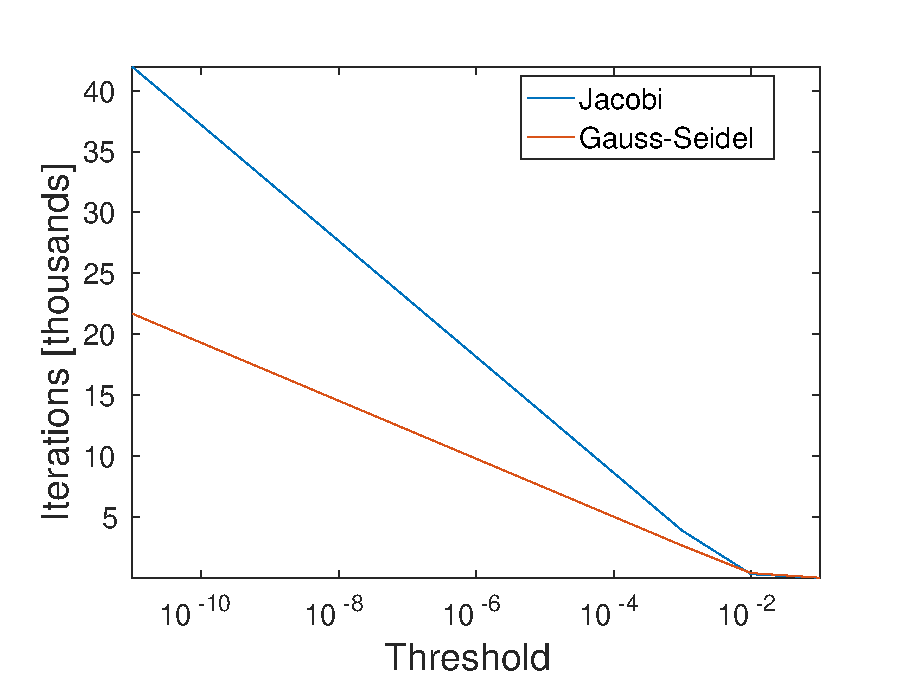
\includegraphics[width = 0.8\textwidth]{fig/itd_jac_gs.eps}
\caption{The convergence of the Jacobi method and the Gauss-Seidel method with changing threshold.}
\label{fig:itd}
\end{figure}


\subsection{OpenMP of the Jacobi Method}

\subsection{Speedup with varying matrix size}
In this subsection, the speedup of the \texttt{omp3} parallelization is investigated with changing matrix sizes. The threshold level is chosen individually for each size such that the program runs for at least a few seconds. The resulting curves can be seen in figure \ref{fig:speedup_N}. Despite the differing thresholds, the curves are still comparable due to the fact that the parallel region is outside the loop in \texttt{omp3}, which means that each iteration is identical, and so a larger number of iterations does not influence the speedup because it is relative to the case with one processor. The number of iterations for a single curve is constant for all number of processors. For a small number of processors, the speedup is similar, but as the number of processors increase, so does the parallel overhead required to keep track of the threads. This limits the speedup, and for a large number of processors, it even decreases for matrix sizes of $N = 500$ and $N = 1000$. For $N = 100$ the quickest is to use one core, simply because the overhead of even two cores takes more time than is gained by the parallelization. For $N = 10000$ the speedup is not seen to decrease because the matrix is so large that the speed gained from the parallelization is larger than the loss from the parallel overhead. If a larger number of cores was available, a decrease in speedup is expected. For $N = 100$, the analyzer tool was used to confirm our hypothesis: For 1 core, the program took $\sim 2.5$ s to run, but for 10 cores, the program spent 39 s on the implicit barriers after the for loops alone, i.e. a lot of work is done to keep track of the synchronization of the threads while the fraction of time where they are actually working is very small. And that is even when the parallel region is outside the main while loop, so the worker team is not destroyed on each iteration, but it is put to sleep and woken up many times, which also affect performance.

\subsection{Speedup with different compiler option}

\begin{figure}
\centering
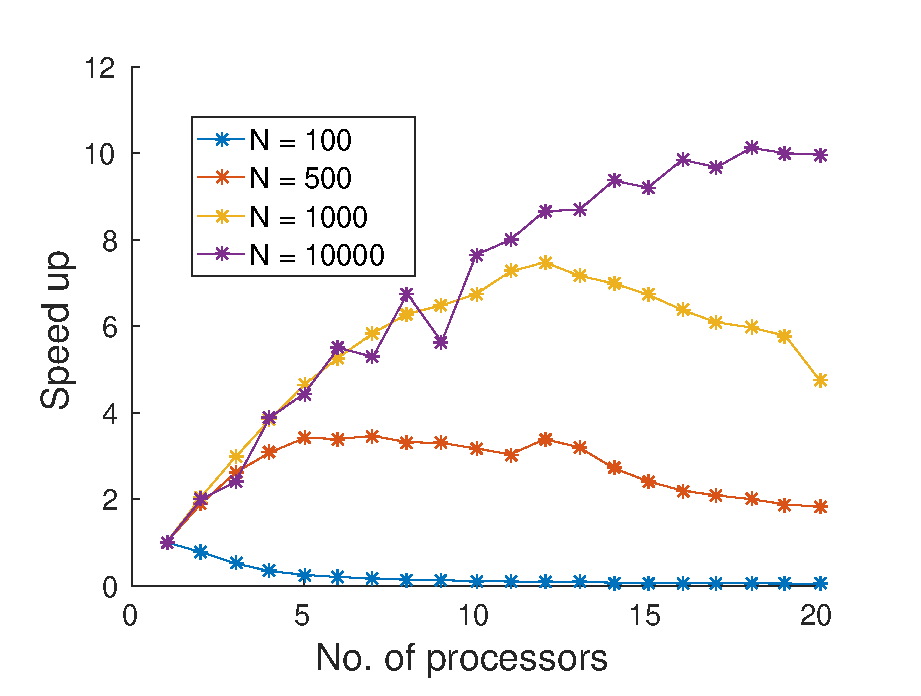
\includegraphics[width = 0.8\textwidth]{fig/speedup_N.eps}
\caption{The speedup of the Jacobi iteration with the best parallellization method, \texttt{omp3}, with different matrix sizes.}
\label{fig:speedup_N}
\end{figure}

\subsection{Comparison with Mandelbrot program}
In this subsection, the scaling of our best parallelized version of the Jacobi method, \texttt{omp3} is compared with the scaling of the computation of the Mandelbrot set.
\section{OpenMP Gauss-Seidel}
The problem with the Gauss-Seidel smoother is, that it is built around internal data dependencies. It is therefore difficult to implement simple parallelized techniques, since the communication cost between the different threads would be really high. The Jacobi method on the other hand uses another matrix, the u old, which takes up memory space, but it is much easier to feed the data to the threads and finish the computation step. Since implementing a parallelization of the Gauss-Seidel smoothening is more difficult, the Jacobi method or alternatives have been more widely used for multigrid problems.\\

There does however exist modifications to the natural/lexographical version of the Gauss-Seidel smoother, which then seeks parallize using different methods, i.e. blocking. The article by D. Wallin, H. L\"{o}f, E. Hagersten and S. Holmgren\footnote{Dan Wallin, Henrik L\"{o}f, Erik Hagersten and Sverker Holmgren, \textit{Multigrid and GaussSeidel
Smoothers Revisited:
Parallelization on Chip Multiprocessors}, ICS '06 Page 145-155, ACM NY USA, 2006-06-28}  give insight to the complications of the subject and describe both the standard red-black method and their new temporally blocked natural Geiss-Seidel smoother. The completely natural Gauss-Seidel is a single sweep for each step/iteration, and therefore the data is interchanged. The red-black ordering is based on splitting each iteration step up in sweeps, which are fully data parallel. The grid is split into sets of even and odd gridpoints, even points have data dependencies to odd points and vice versa. However, the points do not have dependence to points of the same type. This means a loop over points of the same type can be done in parallel. In practice our initial approach would thus likely be to have a loop over one type of points, then a barrier and then a loop over points of the other type.

Their own implementation does blocking as well, but it is not temporal and not strictly like the red-black ordering, which gives the advantage of better cache efficiency for larger matrices compared to the red-black method. Through their work, they succeeded in improving the efficiency up to 40\% compared to some other Gauss-Seidel parallelized smoothers, but it does however depend much on the system and problem at hand.\\

There do exist several possible implementations of the Gauss-Seidel smoother, but it is an evolving field and there exist different approaches. The article by H. Courtecuisse and J. Allard\footnote{Hadrien Courtecuisse, J\'{e}r\'{e}mie Allard, \textit{Parallel Dense Gauss-Seidel Algorithm on Many-Core Processors}, High Performance Computing and Communications, 1th IEEE Conference 2009, IEEE, 2009-06-25} comes with different approaches to the same issue. They present a new parallel dense Gauss-Seidel algorithmn, which is based on atomic update counter, which stores an integer counter in shared memory describing the processed blocks. This depends on the system used, but if it is possible on the system, then after an initial delay, the algorithm will get up to speed without facing the huge communication costs. The article further analyzes this algorithm in depth and its performance across different problem parameters and hardware systems.\\





\section{Conclusion}
In this report, a sequential implementation of the Jacobi iterative method and the Gauss-Seidel iterative method was implemented to solve Poisson's differential equation. The Gauss-Seidel method was found to converge twice as few iterations as the Jacobi method, but in turn the grid point updates per second was slower, but in total, the Gauss-Seidel method was found to be quicker in wall clock time. The Jacobi function can be easily parallelized, so three different versions with increasing amount of parallelization was created. The first only parallelized the loop updating each point, which gave a speedup of maximum 15 \%. Secondly, the checking and the iterative while loop was parallelized, which increased the speedup to a factor of $\sim 4$. Finally, the memory allocation and initialization was parallellized, bringing the top speedup to a factor of 10, which corresponds nicely to $f = 0.955$ in Amdahl's law, suggesting that our code has parallelized over 95 \% of the processes. Using this last implementation, it was found that the optimal number of cores used depends on the matrix size due to increasing parallel overhead from an increasing number of cores. Finally, a method for parallelizing the Gauss-Seidel method is discussed, but not implemented.
\end{document}
